\paragraph{Calculo de Posiciones para los paneles}

Del calculo de la acústica obtuvimos el tiempo de reverberación, de cual se puede calcular la absorción estimada el cuarto. La absorción calculada nos permite calcular, de acuerdo a la absorción de los paneles, la cantidad de superficie que se tiene que añadir al cuarto para alcanzar un tiempo de reverberación deseado. \\
Entonces, resta obtener un programa que a partir de las posiciones de los paneles y la superficie necesaria, nos entregue las nuevas posiciones de los paneles que resulten en la acústica deseada. 

La implementación se hizo en Python y la lógica es la siguiente:
\begin{itemize}
    \item Encontrar el numero de paneles que se deben de cambiar de la posición de reflexión a la posición de absorción, con base en la absorción efectiva del panel y la diferencia entre tiempos de reveberación (actual y deseado)
    \item Si el numero de paneles supera al numero de paneles disponibles, solo mover los disponibles
    \item Preguntar al usuario cuantos de los paneles que no se cambiaran a la posición de absorción quiere cambiar a la posición de difusión. Se deja este proceso al usuario ya que la especialidad no es un parámetro ideal, si no que varia en función al deseo artístico del usuario.
    \item Dada una jerarquía de paneles (primero mover los de en medio, e ir moviéndose hacia los extremos para después terminar los huecos) cambiar el indicador de tipo de panel a absorción y los deseados a difracción.
\end{itemize}

Para encontrar el numero de paneles faltantes, utilizamos la formula de la reverberación: 
\begin{equation}
    RT = \frac{0.161 V}{S \alpha}
\end{equation}
Ya que la frecuencia central utilizada por la mayoría de instrumentos y tratamientos acústicos es a los 500 Hz, se tomara la absorción de los paneles a esta frecuencia. 
\begin{lstlisting}[frame=single,numbers=left, style=matlab-editor, basicstyle=\tiny]
def PanelsToChange(Current_RT60, Needed_RT60, room_dim):
    V = np.prod(room_dim)
    Panel_Surface = np.prod(PanelSize)
    Current_Abs = 0.161*V/Current_RT60
    Needed_Abs = 0.161*V/Needed_RT60
    AbsFromSinglePanel = Panel_Surface*(AbsCoeffs['AbsPanels'][6]-AbsCoeffs['Concrete'][6])
    PanelsToChange = (Needed_Abs-Current_Abs)//AbsFromSinglePanel
    return PanelsToChange

x = PanelsToChange(0.9,0.4,room_dim)
print(f'Changing {int(x)} panels to Absorption')
\end{lstlisting}
Se puede observar que se colocaron los coeficientes de absorción en diccionarios, que se pueden acceder por medio del indicador \textit{string}.
\begin{lstlisting}[frame=single,numbers=left, style=matlab-editor, basicstyle=\tiny]
if x > 18:
    print('Only 18 panels available')
    x = 18

DPanels = int(input(f"Enter the number of diffusion panels to put ({18-x} Available): "))
if DPanels > 18-x :
    print("Not a valid number, using 0")
    DPanels = 0
\end{lstlisting}
Después, se hace la validación de la cantidad de paneles disponibles y, en función de los restantes, la cantidad de paneles de difusión a cambiar.\\
Para la modificación del tipo de panel en función a la jerarquía se decidió utilizar un tipo de estructura llamada \textit{linked list}, ya que nos permitirá guardar los datos del panel (Que tipo de superficie se pondrá y que posición ocupa en el arreglo de paneles) en un nodo, además de poder indicar, cual es el siguiente nodo a visitar. De esta manera, podemos crear una programa que va visitando los paneles en función de la lista jerárquica, la cual sera, el orden de los paneles en la lista. Para el movimiento en si, se puede visitar la lista y obtener los datos del nodo, lo que nos permitirá asociar una posición en arreglo con cierto tipo de panel.
\begin{lstlisting}[frame=single,numbers=left, style=matlab-editor, basicstyle=\tiny]
class Node:
    def __init__(self, data, position):
        self.Type = data
        self.Position = position
        self.next = None
\end{lstlisting}
El nodo solo contiene el tipo de panel (1:'Reflexion',2:'Absorcion',3:'Difraccion'), la posición que ocupa en el arreglo, existen 18 posiciones que indican los 9 paneles que hay por pared, y la referencia al siguiente nodo, el cual nos da la lista jerárquica. \\
El constructor de la lista solo indica cual es la \textit{cabeza} o inicio de la lista y después, se van añadiendo nodos conforme a la lista jerárquica.
\begin{lstlisting}[frame=single,numbers=left, style=matlab-editor, basicstyle=\tiny]
PanelOrder = LinkedList() 
PanelOrder.insertAtBegin(NameToKey['Refle'], 14)
PanelOrder.insertAtEnd(NameToKey['Refle'], 5)
PanelOrder.insertAtEnd(NameToKey['Refle'], 12)
PanelOrder.insertAtEnd(NameToKey['Refle'], 16)
PanelOrder.insertAtEnd(NameToKey['Refle'], 3)
PanelOrder.insertAtEnd(NameToKey['Refle'], 7)
PanelOrder.insertAtEnd(NameToKey['Refle'], 10)
PanelOrder.insertAtEnd(NameToKey['Refle'], 18)
PanelOrder.insertAtEnd(NameToKey['Refle'], 1)
PanelOrder.insertAtEnd(NameToKey['Refle'], 9)
PanelOrder.insertAtEnd(NameToKey['Refle'], 13)
PanelOrder.insertAtEnd(NameToKey['Refle'], 15)
PanelOrder.insertAtEnd(NameToKey['Refle'], 4)
PanelOrder.insertAtEnd(NameToKey['Refle'], 6)
PanelOrder.insertAtEnd(NameToKey['Refle'], 11)
PanelOrder.insertAtEnd(NameToKey['Refle'], 17)
PanelOrder.insertAtEnd(NameToKey['Refle'], 2)
PanelOrder.insertAtEnd(NameToKey['Refle'], 8)
\end{lstlisting}
En la lista jerárquica la prioridad es la siguiente:
\begin{itemize}
    \item (1) Panel central (Posición 5)
    \item (2) Panel izquierdo con uno de separación del central (Posición 3)
    \item (2) Panel derecho con uno de separación del central (Posición 7)
    \item (3) Panel del extremo izquierdo (Posición 1)
    \item (3) Panel del extremo derecho (Posición 9)
    \item (4) Panel izquierdo pegado al central (Posición 4)
    \item (4) Panel derecho pegado al central (Posición 6)
    \item (5) Panel izquierdo pegado al del extremo (Posición 2)
    \item (5) Panel derecho pegado al del extremo (Posición 8)
\end{itemize}
Esta lista jerárquica nos permite mantener el balance de paneles en el cuarto y los paneles con el mismo numero se consideran un conjunto. Cabe resaltar que esta lista es solo para una pared, los de las demás paredes siguen la misma lista jerárquica, con la diferencia que al terminar un conjunto, se modifica ese mismo conjunto en la siguiente pared y posteriormente se vuelve a modificar el siguiente conjunto de la primer pared.
El cambio de tipo de los paneles se hace con el siguiente código:
\begin{lstlisting}[frame=single,numbers=left, style=matlab-editor, basicstyle=\tiny]
for i in range(18):
    if i < x:
        PanelOrder.updateNode(NameToKey['Abs'],i)
    elif i < x + DPanels:
        PanelOrder.updateNode(NameToKey['Scatt'],i) 
    else:
        PanelOrder.updateNode(NameToKey['Refle'],i) 
\end{lstlisting}
Se puede ver como va por la lista jerárquica y cambia los absorbentes, luego los de difracción indicados y los restantes los mantiene en reflexivos. \\
Por ultimo, para acceder a los paneles en orden, se guardan en un diccionario, donde la \textit{key} es la posición en el arreglo (No la lista), y el valor es el tipo de panel en esa posición.
\begin{lstlisting}[frame=single,numbers=left, style=matlab-editor, basicstyle=\tiny]
def GetPanels(PanelOrder):
    PanelArray = {}
    for i in range(18):
        currentPanel_Type, currentPanel_Pos = PanelOrder.returnAtIndex(i)
        PanelArray[currentPanel_Pos] = currentPanel_Type
    return PanelArray

PanelArray = GetPanels(PanelOrder)
for i in range(1,19):
    print(PanelArray[i])
\end{lstlisting}
Iterar a lo largo del diccionario nos da el tipo de panel de cada posición y es el utilizado para el control. \\
Para validarlo, se realizaron varios ejemplos. En el primer caso, se cambiara el tiempo de reverberación de 0.9 s a 0.85 s. El programa calcula que es necesario cambiar dos paneles a absorción y en este caso, se indico que agregara cinco paneles de difusión. La lista de paneles entregada es: $(1,1,3,1,2,1,3,1,1) (3,1,3,1,2,1,3,1,1)$. Se puede observar que solo los paneles centrales se cambiaron a absorción, que los de difracción están balanceados en el arreglo derecho y que el panel de difusión extra en la derecha esta en el extremo izquierdo. \\
\begin{figure}[!htb]
    \centering
    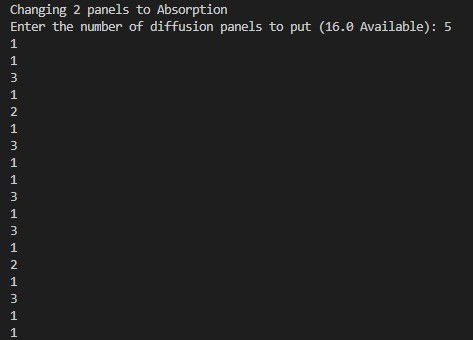
\includegraphics[width=0.8\textwidth]{imagenes/PanelsExample1.jpg}
    \caption{Prueba uno de calculo de posiciones para los paneles}
    \label{fig:PanelsExample1}
\end{figure}
\FloatBarrier
En el segundo caso, se cambiara el tiempo de reverberación de 0.9 s a 0.7 s. El programa calcula que es necesario cambiar doce paneles a absorción y en este caso, se indico que agregara 2 paneles de difusión. La lista de paneles entregada es: $(2,1,2,3,2,3,2,1,2) (2,1,2,2,2,2,2,1,2)$. Se puede observar que en ambos arreglos, los paneles impares se cambiaron a absorción, y los dos sobrantes se colocaron junto al central y se puede ver también que los de difracción están balanceados en el arreglo izquierdo. \\
\begin{figure}[!htb]
    \centering
    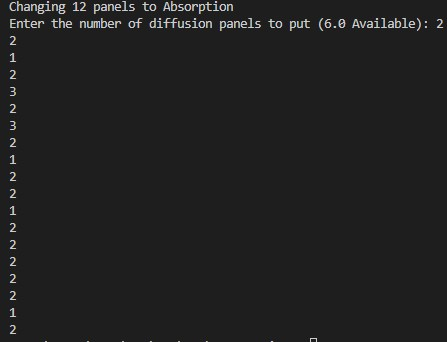
\includegraphics[width=0.8\textwidth]{imagenes/PanelsExample2.jpg}
    \caption{Prueba dos de calculo de posiciones para los paneles}
    \label{fig:PanelsExample2}
\end{figure}
\FloatBarrier
